\documentclass[12pt]{report}

\usepackage{epsf,amsmath,amsfonts}
\usepackage{graphicx}


%\setlength{\textwidth}{6.5in}
%\setlength{\oddsidemargin}{0in}
%\setlength{\evensidemargin}{0in}
%\setlength{\textheight}{9.0in}
%\setlength{\topmargin}{0in}

\setlength{\parskip}{1.2ex}
\setlength{\parindent}{0mm}
\newcommand{\bea}{\begin{eqnarray}}
\newcommand{\eea}{\end{eqnarray}}
\newcommand{\nn}{\nonumber}

\def\ep{\epsilon}
\def\f{\frac}
\def\df{\dfrac}
\def\p{\partial}
\def\tilde{\widetilde}
\def\hat{\widehat}
\def\bs{\boldsymbol}
\def\wh{\widehat}
\def\ud{\,\mathrm{d}}
\def\grad{\nabla}

\def\ub{\mathbf{u}}
\def\vb{\bs{\mathrm{v}}}
\def\Ub{\mathbf{U}}
\def\kb{\bs{\mathrm{k}}}
\def\nb{\bs{\mathrm{n}}}
\def\Kb{\bs{\mathrm{K}}}
\def\Sb{\bs{\mathrm{S}}}


\begin{document}

\title{Mesoscale Eddy Parametrizations \\
with General Vertical Coordinates: \\
Requirements and Design}
\author{MPAS Development Team}

\maketitle
\tableofcontents

%-----------------------------------------------------------------------

\chapter{Summary}

Mesoscale eddy parametrization is an important process in determining the distribution of temperature, salinity and, as a result, density though out the world ocean (\cite{GentMc90, GWMMc95, Gent20}). The purpose of this design process is to implement a MEP into MPAS-Ocean model. Our first goal is a successful implementation of GM.
In the current code, a 'gm' module is available that produces 
a bolus velocity $u^\ast$. The current code also has in place 
the mechanism to add such bolus velocity to the mean transport 
velocity. However, the module can only handle the isopycnal model, 
which is a special case of the general vertical 
coordinate. The new implementation of the GM should calculate 
the bolus velocity and diffusion along isopycnal surfaces from the calculation of isopyncal slopes for use with any vertical coordinate.  
It also includes a tapering process by the means of solving a
vertical boundary value problem. The GM closure has certain well-known
properties, such as mass conservation, sink of potential energy, etc.
The new implementation can be considered a success if it can reproduce
these properties.

%figure template
%\begin{figure}
%  \center{\includegraphics[width=14cm]{./Figure1.pdf}}
%  \caption{A graphical representation of the discrete boundary.}
%  \label{Figure1}
%\end{figure} 




%-----------------------------------------------------------------------

\chapter{Requirements}

\section{Requirement: 1}
Date last modified: 2012/09/06 \\
Contributors: Qingshan Chen and Todd Ringler\\

This implementation of GM should make it possible for MPAS-O to
perform low-resolution (say, 125km) simulations and reproduce model
physics as expected. For example, GM should reduce available potential energy as compared to a run of the same resolution without GM.

\section{Requirement: 2}
Date last modified: 2012/09/06 \\
Contributors: Qingshan Chen and Todd Ringler\\

This implementation of advective portion of GM should be based on a local stream-function formulation so as to make the GM module portable to other ocean models. The stream function formulation guarantees that the bolus velocity is non-divergent.


\section{Requirement: 3}
Date last modified: 2012/09/06 \\
Contributors: Qingshan Chen and Todd Ringler\\

This implementation of GM should involve some ``tapering'' process so
that in regions where the isopycnal surfaces are nearly vertical, the
GM closure should have small coefficients or are essentially shut down.

\section{Requirement: 4}
Date last modified: 2012/09/06 \\
Contributors: Qingshan Chen and Todd Ringler\\

This implementation of GM should be valid for any specification of $\kappa$, the GM closure parameter, i.e. we need to permit $\kappa=f(x,y,z,t)$.

\section{Requirement: 5}
Date last modified: 2012/09/06 \\
Contributors: Qingshan Chen and Todd Ringler\\

This implementation of GM must include a component that allows for the diffusion of tracers along isopycnal surface in a manner generally referred to as Redi diffusion (reference).

%-----------------------------------------------------------------------

\chapter{Algorithmic Formulations}

\section{The model with GM closure on a general vertical coordinate}
Date last modified: 2012/09/06 \\
Contributors: Qingshan Chen and Todd Ringler\\

The thickness and the passive tracer equations of the MPAS-O model read
\begin{align}   
\dfrac{\partial h_k}{\partial t} 
 + \nabla \cdot \left( h_k {\bf u}_k \right) 
% + w^{top}_{k+1} - w^{top}_{k} = 0
 + w_k^\textrm{t} - w_k^\textrm{b} = 0\label{eq:1},
\\
\dfrac{\partial h_k\varphi_k}{\partial t} 
 + \nabla \cdot \left( h_k\varphi_k {\bf u}_k \right) 
%+  w^{top}_{k+1}\varphi^{top}_{k+1} - w^{top}_{k}\varphi^{top}_{k}
  + \varphi_k^\textrm{t} w_k^\textrm{t} - \varphi_k^\textrm{b} w_k^\textrm{b}
= 0.\label{eq:4}
\end{align}
In the above, the superscripts 't' and 'b' denote the top and bottom surfaces,
respectively, of a fluid layer.
The Gent-McWilliams closure replaces the mean transport velocity $\ub$
and $w$ by the effective transport velocity $\Ub$ and $W$,
\begin{align}   
\dfrac{\partial h_k}{\partial t} 
 + \nabla \cdot \left( h_k {\bf U}_k \right) 
% + w^{top}_{k+1} - w^{top}_{k} = 0
 + W_k^\textrm{t} - W_k^\textrm{b} = 0,\label{eq:5}
\\
\dfrac{\partial h_k\varphi_k}{\partial t} 
 + \nabla \cdot \left( h_k\varphi_k{\bf U}_k \right) 
%+  w^{top}_{k+1}\varphi^{top}_{k+1} - w^{top}_{k}\varphi^{top}_{k}
  + \varphi_k^\textrm{t} W_k^\textrm{t} - \varphi_k^\textrm{b} W_k^\textrm{b}  
= \nabla\cdot\left(h_k \Kb \cdot \nabla\varphi_k \right).\label{eq:6}
\end{align}
In the above, the effective transport velocities can be decomposed
into the mean transport velocity and the GM bolus velocities, 
\begin{align}
&{\bf U}_k = u_k + u^\ast_k,\label{eq:7}\\ 
& W_k = w_k + w^\ast_k,\label{eq:8},
\end{align}
and $\Kb$ is the symmetric, $3\times 3$ diffusivity tensor and will be given later in Section
\ref{sec:redi-isopycn-diff}. 

\section{The stream-function formulation of the GM
  parametrizations}\label{sec:stre-funct-form} 
Let 
\begin{equation}
  \label{eq:10}
  \Psi = \bs{\gamma}\times\kb,
\end{equation}
where $\bs{\gamma}$ is a horizontal 2D vector and $\kb$ is the
vertical unit vector. Let 
\begin{equation}
  \label{eq:2}
  \vb \equiv (\ub^\ast,\,w^\ast) = \nabla_3 \times\Psi.
\end{equation}
Then we find that 
\begin{align}
  &\ub^\ast = \p_z\bs{\gamma},\label{eq:13}\\
 &w^\ast = -\nabla_z\cdot\bs{\gamma}.\label{eq:14}
\end{align}
Now let 
\begin{equation}
  \label{eq:11}
  \bs{\gamma}_\textrm{GM} = -\kappa\Sb,
\end{equation}
where $\Sb$ is a 2D vector representing the slope of the neutral
surfaces, and it is given by 
\begin{equation}
  \label{eq:9}
  \Sb = -\dfrac{\nabla_z \rho}{\rho_z}.
\end{equation}
Here we are approximating neutral surfaces based on the slope 
of $\rho$, the potential density. 
Then
\begin{align}
  &\ub^\ast_\textrm{GM} = -\p_z(\kappa\Sb),  \label{eq:12}\\
  &w^\ast_\textrm{GM} = \nabla_z\cdot(\kappa \Sb).
\end{align}
We note that $w^\ast$ can be determined via (\ref{eq:14}) or using
(\ref{eq:13}) along with the incompressibility constraint
\begin{equation}
  \label{eq:2}
  \nabla \cdot \vb = 0. 
\end{equation}


\section{Tapering by solving a boundary value
  problem}\label{sec:taper-solv-bound}  
Following \cite{Ferrari10}, one solves a boundary value
problem for the horizontal 2D vector
$\bs{\gamma}$ in \eqref{eq:13} and \eqref{eq:14},
\begin{align}
  &\left( c^2\dfrac{\ud^2}{\ud z^2} - N^2\right)\bs{\gamma} =
  (g/\rho_0)\kappa \nabla_z\rho,\label{eq:15}\\
  &\bs{\gamma}(\eta) = \bs{\gamma}(-H) = 0.\label{eq:3}
\end{align}
In the above, $c$ is a depth independent speed to be specified,
$\kappa$ is associated with the barotropic eddy stirring, and
therefore is also depth independent. $N^2$ is the Brunt-Vasalai
frequencies, and is give by $N^2 = -(g/\rho_0)\p_z\rho$. We note that,
when $c\longrightarrow 0$, the solution of \eqref{eq:15} and
\eqref{eq:3} reduces to $\bs{\gamma}_\textrm{GM}$, except in the top
and bottom thin boundary layers where $\bs{\gamma}$ goes to zero
while $\bs{\gamma}_\textrm{GM}$ does not.

MPAS-O utilizes a C-grid staggering technique. Hence it is necessary
to recast the full continuous GM formulation, given in the previous
section, in terms of the normal components of the variables. In what
follows, we denote the normal components of $\ub^\ast$ and
$\bs{\gamma}$ by $u^\ast$ and $\gamma$, respectively, i.e.
\begin{align}
  &u^\ast = \ub^\ast\cdot\nb,\label{eq:16}\\
  &\gamma = \bs{\gamma}\cdot\nb,\label{eq:17}
\end{align}
where $\nb$ denotes the outer normal unit vector on the cell
edges. The relation between $u^\ast$ and $\gamma$ is derived by
taking dot-product of \eqref{eq:13} with $\ub$,
\begin{equation}
  \label{eq:18}
  u^\ast = \p_z \gamma.
\end{equation}
We obtain a boundary value problem for the normal component $\gamma$ by
taking dot-product of \eqref{eq:15}--~\eqref{eq:3} with $\nb$,
\begin{align}
  &\left( c^2\dfrac{\ud^2}{\ud z^2} - N^2\right){\gamma} =
  \left.(g/\rho_0)\kappa \dfrac{\p \rho}{\p \mathrm{n}}\right|_z,\label{eq:19}\\
  &{\gamma}(\eta) = {\gamma}(-H) = 0.\label{eq:20}
\end{align}
Here $(\p \rho/\p\mathrm{n})|_z$ refers to the normal derivative of
the potential density field on constant height surfaces.

% \section{Formulae}\label{sec:formulae}
% Date last modified: 2012/09/21 \\
% Contributors: Qingshan Chen and Todd Ringler\\

The calculation of $\p\rho/\p\mathrm{n}$ on constant height surfaces is 
a bit more complicated, because the general vertical coordinate
usually 
does not align with the traditional $z$-level coordinate. We begin by 
deriving a formula for $\nabla_z\rho$ on the general
coordinate. Projecting $\nabla_z\rho$ in the direction of $\nb$ will
give $\p\rho/\p\mathrm{n}$ on  
constant height surfaces.
We call the general vertical coordinate $r$. Thus it can be written that 
\begin{align}
& r = r(x,y,z),\label{eq:22}\\
& z = z(x,y,r).\label{eq:23}
\end{align}
The time variable $t$ has been dropped for now, since it is not relevant
in the derivation. Applying the horizontal gradient operator $\nabla_z$ 
to $\rho(x,y,r(x,y,z))$, and using the chain rule, we obtain
\begin{equation}
\nabla_z \rho = \nabla_r\rho + \dfrac{\p\rho}{\p r}\nabla_z r.
\label{eq:24}
\end{equation}
Applying $\nabla_z$ to \eqref{eq:23}, we obtain
\begin{equation*}
0 = \nabla_r z + \dfrac{\p z}{\p r}\nabla_z r.
\end{equation*}
Hence
\begin{equation}
\nabla_z r = \frac{-\nabla_r z}{\frac{\p z}{\p r}}.\label{eq:25}
\end{equation}
Applying $\p/\p z$ to \eqref{eq:23}, we have
\begin{equation}
1 = \dfrac{\p z}{\p r}\dfrac{\p r}{\p z}.\label{eq:26}
\end{equation}
Combining \eqref{eq:24}--\eqref{eq:26} yields
\begin{equation}
\nabla_z \rho = \nabla_r \rho - \dfrac{\p \rho}{\p r}
\dfrac{\p r}{\p z}\nabla_r z.\label{eq:27}
\end{equation}
We notice that 
\begin{equation}
\dfrac{\p \rho}{\p z} = \dfrac{\p \rho}{\p r}
\dfrac{\p r}{\p z}\label{eq:28}
\end{equation}
by taking the $z$-derivative of $\rho(x,y,r(x,y,z))$. Hence 
\eqref{eq:27} can be written as
\begin{equation}
\nabla_z \rho = \nabla_r \rho - \dfrac{\p\rho}{\p z}\nabla_r z.
\label{eq:29}
\end{equation}
Taking dot-product of \eqref{eq:29} with the outer normal unit vector
$\nb$ yields
\begin{equation}
\left.\dfrac{\p\rho}{\p \mathrm{n}}\right|_z = 
\left.\dfrac{\p\rho}{\p\mathrm{n}}\right|_r - \left.\dfrac{\p\rho}{\p z}
\dfrac{\p z}{\p\mathrm{n}}\right|_r.
\label{eq:30}
\end{equation}


\section{Redi, along-neutral-surface diffusion}\label{sec:redi-isopycn-diff} 
Date last modified: 2012/11/19 \\
Contributors: Qingshan Chen, Todd Ringler, and Peter Gent\\


\begin{figure}[h]
  \centering
  \scalebox{0.7}{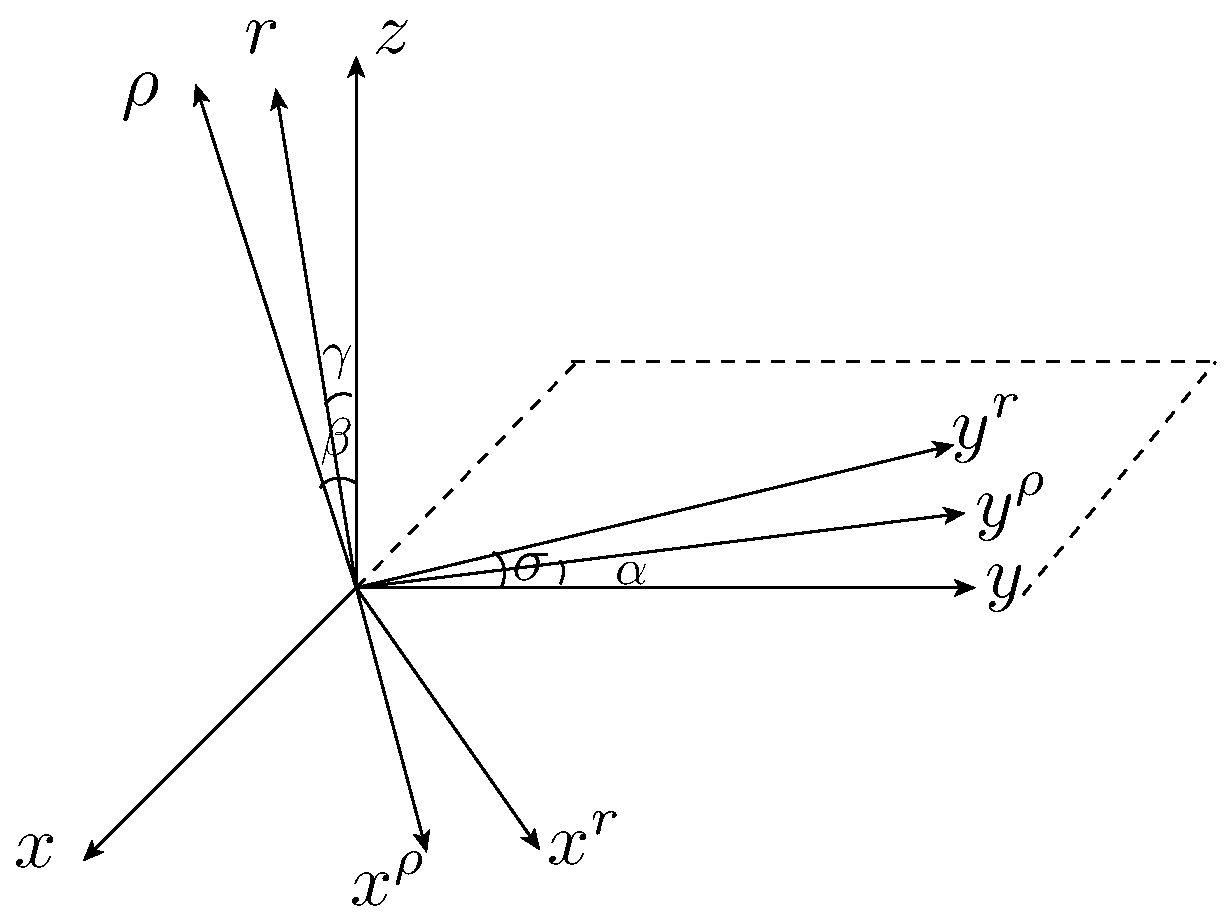
\includegraphics{coordinates.pdf}}
  \caption{Coordinates transformation. Both $y^r$ and $y^\rho$ are on
    the $xy$-plane. The $x^\rho y^\rho\rho$-coordinates can be reached
  by first rotating the $xyz$-coordinates along the $z$-axis
  counter-clockwise by angle $\alpha$, and then rotating the
  intermediate coordinates along $y^\rho$-axis clockwise by angle
  $\beta$. The coordinates $x^ry^rr$-coordinates can be reached
  through a similar process. }
\end{figure}
The transformation between $(x^\rho, y^\rho, \rho)$ and $(x, y, z)$ is
an orthonormal rotation determined by the two angular parameters
$\alpha$ and $\beta$. Specifically, 
\begin{equation}
  \label{eq:21}
  \left(\begin{matrix} x\\ \\ y\\ \\ z\end{matrix}\right) = 
  \left(\begin{matrix}\cos\beta\cos\alpha & -\sin\alpha &
      -\sin\beta\cos\alpha \\ \\
  \cos\beta\sin\alpha & \cos\alpha & -\sin\beta\sin\alpha \\ \\
  \sin\beta & 0 & \cos\beta\end{matrix}\right) 
  \left(\begin{matrix}x^\rho \\ \\ y^\rho \\ \\
      \rho\end{matrix}\right) \equiv M_1  \left(\begin{matrix}x^\rho
      \\ \\ y^\rho \\ \\ \rho\end{matrix}\right) . 
\end{equation}
Similarly, 
\begin{equation}
\label{eq:31}
  \left(\begin{matrix} x\\ \\ y\\ \\ z\end{matrix}\right) = 
  \left(\begin{matrix}\cos\gamma\cos\sigma & -\sin\sigma &
      -\sin\gamma\cos\sigma \\ \\
  \cos\gamma\sin\sigma & \cos\sigma & -\sin\gamma\sin\sigma \\ \\
  \sin\gamma & 0 & \cos\gamma\end{matrix}\right) 
  \left(\begin{matrix}x^r \\ \\ y^r \\ \\ r\end{matrix}\right) \equiv
  M_2 \left(\begin{matrix}x^r \\ \\ y^r \\ \\ r\end{matrix}\right).
\end{equation}
For orthonormal matrices, their inverses are simply their
transposes. Hence, from \eqref{eq:31},
\begin{equation}
\label{eq:32}
  \left(\begin{matrix} x^r\\ \\ y^r\\ \\ r\end{matrix}\right) =
  M_2^\textrm{T} \left(\begin{matrix}x \\ \\ y \\ \\
      z\end{matrix}\right) =
  \left(\begin{matrix}\cos\gamma\cos\sigma & \cos\gamma\sin\sigma &
      \sin\gamma \\ \\
  -\sin\sigma & \cos\sigma & 0\\ \\
  -\sin\gamma\cos\sigma & -\sin\gamma\sin\sigma &
  \cos\gamma\end{matrix}\right)  
  \left(\begin{matrix}x \\ \\ y \\ \\ z\end{matrix}\right).
\end{equation}
Combining \eqref{eq:21} and \eqref{eq:32}, one obtains the
transformation from the density ($\rho$) coordinate system to the
general ($r$) coordinate system,
\begin{equation}
\label{eq:33}
  \left(\begin{matrix} x^r\\ \\ y^r\\ \\ r\end{matrix}\right) =
  M_2^\textrm{T} M_1\left(\begin{matrix}x^\rho \\ \\ y^\rho \\ \\
      \rho\end{matrix}\right) \equiv M_3\left(\begin{matrix}x^\rho \\
      \\ y^\rho \\ \\ \rho\end{matrix}\right).
\end{equation}
%The matrix multiplication is carried out with the symbolic algebraic
%system $Mathematica^\textrm{TM}$, and the resulting transformation
%matrix $M_3$ is given below in Mathematica format:
%\begin{multline}
%M_3 = \{\{\text{Cos}[\alpha ] \text{Cos}[\beta ]
%  \text{Cos}[\gamma ] \text{Cos}[\sigma ]+\text{Sin}[\beta ]
%  \text{Sin}[\gamma ]+\text{Cos}[\beta ] \text{Cos}[\gamma ]
%  \text{Sin}[\alpha ] \text{Sin}[\sigma ],\\
%-\text{Cos}[\gamma ]
%  \text{Cos}[\sigma ] \text{Sin}[\alpha ]+\text{Cos}[\alpha ]
%  \text{Cos}[\gamma ] \text{Sin}[\sigma ],\\
%-\text{Cos}[\alpha ]
%  \text{Cos}[\gamma ] \text{Cos}[\sigma ] \text{Sin}[\beta
%  ]+\text{Cos}[\beta ] \text{Sin}[\gamma ]-\text{Cos}[\gamma ]
%  \text{Sin}[\alpha ] \text{Sin}[\beta ] \text{Sin}[\sigma
%  ]\},\\
%\{\text{Cos}[\beta ] \text{Cos}[\sigma ] \text{Sin}[\alpha
%  ]-\text{Cos}[\alpha ] \text{Cos}[\beta ] \text{Sin}[\sigma
%  ],\text{Cos}[\alpha ] \text{Cos}[\sigma ]+\text{Sin}[\alpha ]
%  \text{Sin}[\sigma ],\\
%-\text{Cos}[\sigma ] \text{Sin}[\alpha ]
%  \text{Sin}[\beta ]+\text{Cos}[\alpha ] \text{Sin}[\beta ]
%  \text{Sin}[\sigma ]\},\\
%\{\text{Cos}[\gamma ] \text{Sin}[\beta
%  ]-\text{Cos}[\alpha ] \text{Cos}[\beta ] \text{Cos}[\sigma ]
%  \text{Sin}[\gamma ]-\text{Cos}[\beta ] \text{Sin}[\alpha ]
%  \text{Sin}[\gamma ] \text{Sin}[\sigma ],\\
%\text{Cos}[\sigma ]
%  \text{Sin}[\alpha ] \text{Sin}[\gamma ]-\text{Cos}[\alpha ]
%  \text{Sin}[\gamma ] \text{Sin}[\sigma ],\\
%\text{Cos}[\beta ]
%  \text{Cos}[\gamma ]+\text{Cos}[\alpha ] \text{Cos}[\sigma ]
%  \text{Sin}[\beta ] \text{Sin}[\gamma ]+\text{Sin}[\alpha ]
%  \text{Sin}[\beta ] \text{Sin}[\gamma ] \text{Sin}[\sigma ]\}\} 
%\end{multline}
The transformation $M$ from the density $\rho$ coordinate system to the
hybrid curvelinear $(x,y,r)$ coordinate system is obtained by
combining relevant rows from matrices $M_1$ and $M_3$. Specifically,
using the Matlab conventions,
\begin{align}
  \label{eq:34}
  M = \left(
    \begin{aligned}
     &M_1(1,:)\\
     &M_1(2,:)\\
     &M_3(3,:)
    \end{aligned}\right),
\end{align}
and
\begin{equation}
\label{eq:35}
  \left(\begin{matrix} x\\ \\ y\\ \\ r\end{matrix}\right) =
  M\left(\begin{matrix}x^\rho \\
      \\ y^\rho \\ \\ \rho\end{matrix}\right).
\end{equation}

Let $\varphi = \varphi(x^\rho, y^\rho, \rho,t) = \varphi(x,y,r,t)$ be
some tracer. Then, using chain rules, one has
\begin{equation}
\label{eq:36}
  \left(\begin{matrix}\frac{\p\varphi}{\p x^\rho}\\ \\
      \frac{\p\varphi}{\p y^\rho} \\ \\ \frac{\p\varphi}{\p
        \rho} \end{matrix}\right)= 
  \left(\begin{matrix}\frac{\p x}{\p x^\rho} & \frac{\p y}{\p x^\rho} &
      \frac{\p r}{\p x^\rho} \\ \\
\frac{\p x}{\p y^\rho} & \frac{\p y}{\p y^\rho} &
     \frac{\p r}{\p y^\rho} \\ \\
\frac{\p x}{\p \rho} & \frac{\p y}{\p\rho} &
    \frac{\p r}{\p\rho} 
\end{matrix}\right)  
  \left(\begin{matrix}\frac{\p\varphi}{\p x}\\ \\
      \frac{\p\varphi}{\p y} \\ \\ \frac{\p\varphi}{\p
        r} \end{matrix}\right).
\end{equation}
Using \eqref{eq:35}, one can write \eqref{eq:36} as
\begin{equation}
\label{eq:37}
  \left(\begin{matrix}\frac{\p\varphi}{\p x^\rho}\\ \\
      \frac{\p\varphi}{\p y^\rho} \\ \\ \frac{\p\varphi}{\p
        \rho} \end{matrix}\right)= 
  M^\textrm{T}
  \left(\begin{matrix}\frac{\p\varphi}{\p x}\\ \\
      \frac{\p\varphi}{\p y} \\ \\ \frac{\p\varphi}{\p
        r} \end{matrix}\right).
\end{equation}

In the density coordinate system $(x^\rho, y^\rho, \rho)$, the
diffusion of the tracer can be formulated as
\begin{equation}
  \label{eq:38}
  \nabla^\rho\cdot(K^\rho\nabla^\rho\varphi),
\end{equation}
where $\nabla^\rho = (\p_{x_\rho}, \p_{y_\rho}, \p_\rho)^\textrm{T}$, and $K^\rho$
denotes a tensor. The assumption that tracer diffusion should be along
instead of across isopycnal surfaces can be realized by setting the
diffusion tensor to
\begin{equation}
  \label{eq:39}
  K^\rho = \kappa_R \left(
    \begin{matrix}
      1 & 0 & 0\\
      0 & 1 & 0\\
      0 & 0 & 0
    \end{matrix}\right)
\end{equation}
where $\kappa_R$ is the Redi, along-neutral-surface diffusivity.
Using the relation \eqref{eq:37}, one can formulate the diffusion
\eqref{eq:38} in the general hybrid coordinate system $(x, y, r)$ as
\begin{equation}
  \label{eq:40}
  \nabla^r\cdot(K^r\nabla^r\varphi) \equiv  \nabla^r\cdot(MK^\rho
  M^\textrm{T}\nabla^r\varphi), 
\end{equation}
where $\nabla^r = (\p_x, \p_y, \p_r)^\textrm{T}$. With $K^\rho$ taking
the form in \eqref{eq:39}, 
%the new tensor $K^r$ can be easily found
%using Mathematica,
%\begin{multline}
%  \label{eq:41}
%  K^r = \{\{\text{Cos}[\alpha ]^2 \text{Cos}[\beta
 %     ]^2+\text{Sin}[\alpha ]^2,\\
   %   -\text{Cos}[\alpha ] \text{Sin}[\alpha
  %    ]+\text{Cos}[\alpha ] \text{Cos}[\beta ]^2 \text{Sin}[\alpha
  %    ],\\
  %    \text{Cos}[\alpha ] \text{Cos}[\beta ] \text{Cos}[\gamma ]
  %    \text{Sin}[\beta ]-\text{Cos}[\alpha ]^2 \text{Cos}[\beta ]^2
  %    \text{Cos}[\sigma ] \text{Sin}[\gamma ]-\\
 %     \text{Cos}[\sigma ]
 %     \text{Sin}[\alpha ]^2 \text{Sin}[\gamma ]+
 %     \text{Cos}[\alpha ]
  %    \text{Sin}[\alpha ] \text{Sin}[\gamma ] \text{Sin}[\sigma
  %    ]-\text{Cos}[\alpha ] \text{Cos}[\beta ]^2 \text{Sin}[\alpha ]
%      \text{Sin}[\gamma ] \text{Sin}[\sigma
 %     ]\},\\
 %     \{-\text{Cos}[\alpha ] \text{Sin}[\alpha
 %     ]+\text{Cos}[\alpha ] \text{Cos}[\beta ]^2 \text{Sin}[\alpha
  %    ],\\
  %    \text{Cos}[\alpha ]^2+\text{Cos}[\beta ]^2 \text{Sin}[\alpha
  %    ]^2,\\
  %    \text{Cos}[\beta ] \text{Cos}[\gamma ] \text{Sin}[\alpha ]
  %    \text{Sin}[\beta ]+\text{Cos}[\alpha ] \text{Cos}[\sigma ]
  %    \text{Sin}[\alpha ] \text{Sin}[\gamma ]-\\
  %    \text{Cos}[\alpha ]
  %    \text{Cos}[\beta ]^2 \text{Cos}[\sigma ] \text{Sin}[\alpha ]
   %   \text{Sin}[\gamma ]-\text{Cos}[\alpha ]^2 \text{Sin}[\gamma ]
   %   \text{Sin}[\sigma ]-\text{Cos}[\beta ]^2 \text{Sin}[\alpha ]^2
 %     \text{Sin}[\gamma ] \text{Sin}[\sigma
   %   ]\},\\
 %     \{\text{Cos}[\alpha ] \text{Cos}[\beta ]
 %     \text{Cos}[\gamma ] \text{Sin}[\beta ]-\text{Cos}[\alpha ]^2
 %     \text{Cos}[\beta ]^2 \text{Cos}[\sigma ] \text{Sin}[\gamma
 %     ]-\\
  %    \text{Cos}[\sigma ] \text{Sin}[\alpha ]^2 \text{Sin}[\gamma
  %    ]+\text{Cos}[\alpha ] \text{Sin}[\alpha ] \text{Sin}[\gamma ]
  %    \text{Sin}[\sigma ]-\text{Cos}[\alpha ] \text{Cos}[\beta ]^2
  %    \text{Sin}[\alpha ] \text{Sin}[\gamma ] \text{Sin}[\sigma
  %    ],\\
  %    \text{Cos}[\beta ] \text{Cos}[\gamma ] \text{Sin}[\alpha ]
  %    \text{Sin}[\beta ]+\text{Cos}[\alpha ] \text{Cos}[\sigma ]
  %    \text{Sin}[\alpha ] \text{Sin}[\gamma ]-\\
  %    \text{Cos}[\alpha ]
  %    \text{Cos}[\beta ]^2 \text{Cos}[\sigma ] \text{Sin}[\alpha ]
  %    \text{Sin}[\gamma ]-\text{Cos}[\alpha ]^2 \text{Sin}[\gamma ]
  %    \text{Sin}[\sigma ]-\text{Cos}[\beta ]^2 \text{Sin}[\alpha ]^2
  %    \text{Sin}[\gamma ] \text{Sin}[\sigma ],\\
   %   \text{Cos}[\gamma ]^2
 %     \text{Sin}[\beta ]^2-2 \text{Cos}[\alpha ] \text{Cos}[\beta ]
   %   \text{Cos}[\gamma ] \text{Cos}[\sigma ] \text{Sin}[\beta ]
 %     \text{Sin}[\gamma ]+\\
 %     \text{Cos}[\alpha ]^2 \text{Cos}[\beta ]^2
  %    \text{Cos}[\sigma ]^2 \text{Sin}[\gamma ]^2+\text{Cos}[\sigma
  %    ]^2 \text{Sin}[\alpha ]^2 \text{Sin}[\gamma ]^2-\\
  %    2\text{Cos}[\beta ] \text{Cos}[\gamma ] \text{Sin}[\alpha ]
   %   \text{Sin}[\beta ] \text{Sin}[\gamma ] \text{Sin}[\sigma ]-2
  %    \text{Cos}[\alpha ] \text{Cos}[\sigma ] \text{Sin}[\alpha ]
  %    \text{Sin}[\gamma ]^2 \text{Sin}[\sigma ]+\\
   %   2 \text{Cos}[\alpha ]
  %    \text{Cos}[\beta ]^2 \text{Cos}[\sigma ] \text{Sin}[\alpha ]
  %    \text{Sin}[\gamma ]^2 \text{Sin}[\sigma ]+\\
  %    \text{Cos}[\alpha ]^2
  %    \text{Sin}[\gamma ]^2 \text{Sin}[\sigma ]^2+\text{Cos}[\beta ]^2
   %   \text{Sin}[\alpha ]^2 \text{Sin}[\gamma ]^2 \text{Sin}[\sigma
   %   ]^2\}\} 
%\end{multline}
We denote by $k_x$ and $k_y$ the slopes of the potential density
surfaces along the $x$ and $y$ axes, respectively, and by $l_x$ and
$l_y$ the slopes of the constant $r$ surfaces along the $x$ and $y$
axes respectively. We also note the following relations,
\begin{align}\
  &k_x = \cos\alpha\tan\beta, & &k_y =
  \sin\alpha\tan\beta,  \label{eq:42}\\
  &l_x = \cos\sigma\tan\gamma, & &l_y =
  \sin\sigma\tan\gamma  \label{eq:43}
 \end{align}
Then the tensor matrix $K^r$ can be written as 
\begin{equation}
  \label{eq:44}
  K^r = \kappa_R \cos^2\beta\left(
    \begin{matrix}
      1 + k_y^2 & { }  &  -k_xk_y & { } & { }\\
          { }   &     { }   & { } & { } & \cos\gamma{\tilde{\mathbf{S}}}\\
      -k_xk_y & { } & 1 + k_x^2 & { } & { }\\
         { } & { } & { } & { } & { } \\
         { } & \cos\gamma\tilde{\mathbf{S}}^\textrm{T} & { } & { } &
         \cos^2\gamma K_{33}
    \end{matrix}\right),
\end{equation}
with 
\begin{align*}
&  \tilde{\Sb} = \left(k_x- l_x + k_y(k_xl_y - k_yl_x),\, k_y-l_y
    + k_x(k_yl_x - k_xl_y)\right)^\textrm{T},\\
&K_{33} = (k_x - l_x)^2 + (k_y - l_y)^2 + (k_yl_x - k_xl_y)^2.
% l_x^2(1+k_y^2) + l_y^2(1+k_x^2) - 2(k_xl_x + k_yl_y) + k_x^2
% + k_y^2 - 2k_xk_yl_xl_y.
\end{align*}
Note that both $\tilde{\Sb}$ and $K_{33}$ are non-dimensional.

In the case when the $(x^r, y^r, r)$-coordinate system coincides with
the $(x,y,z)$-coordinate system, ones $\sigma=\gamma=0$, and hence
$l_x = l_y=0$ according to \eqref{eq:43}. Therefore, $K^r$ reduces to
\begin{equation*}
\kappa_R \cos^2\beta\left(
    \begin{matrix}
      1 + k_y^2 & { }  &  -k_xk_y & { } & {k_x }\\
          { }   &     { }   & { } & { } & { }\\
      -k_xk_y & { } & 1 + k_x^2 & { } & {k_y }\\
         { } & { } & { } & { } & { } \\
         {k_x} & { } & {k_y } & { } & k_x^2 + k_y^2
    \end{matrix}\right),
\end{equation*}
which is exactly the form of the Redi diffusion tensor on the
traditional $z$-level coordinate. In the case when the constant $r$
surface coincides with the constant density $\rho$ surface, one has
$l_x = k_x$ and $l_y=k_y$. Therefore, $K^r$ reduces to 
\begin{equation*}
\kappa_R \cos^2\beta\left(
    \begin{matrix}
      1 + k_y^2 & { }  &  -k_xk_y & { } & { 0 }\\
          { }   &     { }   & { } & { } & { }\\
      -k_xk_y & { } & 1 + k_x^2 & { } & {0 }\\
         { } & { } & { } & { } & { } \\
         {0} & { } & {0 } & { } & 0
    \end{matrix}\right).
\end{equation*}
In this case, the requirement that there should be no flux across the
constant density surface carries over to the constant $r$ surface. The
extra terms in the upper-left $2\times 2$ matrix are due to the fact
that the horizontal $(x,y)$-, instead of $(x^\rho, y^\rho)$-,
coordinate system are used. \\

\subsection{Calculation the local slope of neutral surfaces}
We note that 
\begin{align*}
  (k_x, k_y) &= -\dfrac{\nabla_z\rho}{\rho_z}\\
                &= -\dfrac{1}{\rho_z}\left(\nabla_r\rho +
                  \dfrac{\p\rho}{\p r}\nabla_z r\right)\\
                &= -\dfrac{1}{\rho_z}\left(\nabla_r\rho -
                  \dfrac{\p\rho}{\p z}\nabla_r z\right)\\
                &= -\dfrac{1}{\rho_z}\nabla_r\rho + \nabla_r z.
\end{align*}
That is,
\begin{equation}
  \label{eq:45}
(k_x,k_y) = -\dfrac{1}{\rho_z}\nabla_r\rho + \nabla_r z.
\end{equation}
By definition, the slope of the constant $r$ surface is by
\begin{equation}
  \label{eq:46}
  (l_x, l_y) = \nabla_r z
\end{equation}
Using \eqref{eq:45} and \eqref{eq:46}, the vector $\tilde{\Sb}$ can
written as 
\begin{equation}
  \label{eq:47}
  \tilde{\Sb} = -\dfrac{\nabla_r\rho}{\rho_z} +
  \left( k_y(k_xl_y - k_yl_x),\, k_x(k_yl_x - k_xl_y)\right)^\textrm{T}. 
\end{equation}
The term $K_{33}$ can be written as
% \begin{align*}
%   K_{33} &= (k_x-l_x)^2 + (k_y - l_y)^2 + l_x^2k_y^2 + l_y^2k_x^2 -
%   2k_xk_yl_xl_y\\
%   &= \dfrac{|\nabla_r\rho|^2}{\rho_z^2}+ l_x^2k_y^2 + l_y^2k_x^2 -
%   2k_xk_yl_xl_y.
% \end{align*}
% Hence,
\begin{equation}
  \label{eq:49}
   K_{33} = \dfrac{|\nabla_r\rho|^2}{\rho_z^2}+ (k_yl_x - k_xl_y)^2.
\end{equation}

\subsection{Small angle approximation}
The slopes of the constant density surfaces are usually small,
i.e.~$k_x$ and $k_y$ in \eqref{eq:47} and \eqref{eq:49} are usually
small.  The high order terms involving $k_x$ and/or $k_y$ are even
smaller, and in practice they may be neglected, leading to simpler forms
of the Redi diffusion tensor. We propose to neglect the second-order
terms in the upper-left $2\times 2$ sub-matrix, the third-order
terms of \eqref{eq:47} and the fourth-order terms in \eqref{eq:49},
that is, we take
\begin{equation}
  \label{eq:53}
  K^r = \kappa_R \left(\begin{matrix}
  I_2 & { } & \cos\gamma\tilde{\Sb}\\
\\
  \cos\gamma\tilde{\mathbf{S}} & { } & \cos^2\gamma K_{33}\end{matrix}\right), 
\end{equation}
with
\begin{align}
  &\tilde{\mathbf{S}} =
  -\dfrac{\nabla_r\rho}{\rho_z}, \label{eq:51}\\ 
   &K_{33} = \dfrac{|\nabla_r\rho|^2}{\rho_z^2}\label{eq:52}
 \end{align}
It can be easily checked that the diffusion tensor $K^r$ with
$\tilde{\mathbf{S}}$ and $K_{33}$ taking the simplified forms \eqref{eq:51}
and \eqref{eq:52} has no effect on the density field, that is,
\begin{displaymath}
  K^r\nabla^r\rho = 0.
\end{displaymath}

\subsection{Weak cross-isopycnal-surface diffusion}
If weak cross-isopycnal-surface diffusion is to be considered, then
$K^\rho$ takes the form
\begin{equation}
\label{eq:48}
  K^\rho = \kappa_R \left(
    \begin{matrix}
      1 & 0 & 0\\
      0 & 1 & 0\\
      0 & 0 & \epsilon
    \end{matrix}\right).
\end{equation}
for a small positive, non-dimensional, number $\epsilon$ that represents the ratio of the cross-neutral 
surface mixing to the along-neutral surface mixing. Through the same transformation
given in \eqref{eq:40}, $K^r$ is found to be
\begin{equation}
\label{eq:50}
  K^r = \kappa_R \cos^2\beta\left(
    \begin{matrix}
      1 + k_y^2 + \epsilon k_x^2& { }  &  -(1-\epsilon)k_xk_y & { } & { }\\
          { }   &     { }   & { } & { } & \cos\gamma{\tilde{\mathbf{S}}}\\
      -(1-\epsilon)k_xk_y & { } & 1 + k_x^2+\epsilon k_y^2 & { } & { }\\
         { } & { } & { } & { } & { } \\
         { } & \cos\gamma\tilde{\mathbf{S}}^\textrm{T} & { } & { } &
         \cos^2\gamma K_{33}
    \end{matrix}\right),
\end{equation}
with $\tilde S$ and $K_{33}$ taking the forms
\begin{equation*}
 \tilde{\Sb} = \left(\begin{matrix}k_x- l_x -\epsilon k_x + k_y(k_xl_y - k_yl_x) -
  \epsilon k_x(k_xl_x+k_yl_y) \\
 \\ 
  k_y-l_y - \epsilon k_y
    + k_x(k_yl_x - k_xl_y) - \epsilon
    k_y(k_xl_x+k_yl_y)\end{matrix}\right),
\end{equation*}
and 
\begin{multline*}
K_{33} = (k_x - l_x)^2 + (k_y - l_y)^2 +\epsilon +  (k_yl_x - k_xl_y)^2 + 
2\epsilon(k_xl_x+k_yl_y) + \epsilon(k_xl_x+k_yl_y)^2.
% l_x^2(1+k_y^2) + l_y^2(1+k_x^2) - 2(k_xl_x + k_yl_y) + k_x^2
% + k_y^2 - 2k_xk_yl_xl_y.
\end{multline*}
With the small-angle  approximation, $K^r$ takes the same form as in
\eqref{eq:53}, and $\tilde{S}$ and $K_{33}$ are reduced to 
\begin{equation}
\label{eq:56}
 \tilde{\Sb} = \left(\begin{matrix}k_x- l_x - \epsilon k_x \\
 \\ 
  k_y-l_y - \epsilon k_y
  \end{matrix}\right) =  -(1-\epsilon)\dfrac{\nabla_r\rho}{\rho_z} - 
  \epsilon\nabla_r z,
\end{equation}
and 
\begin{equation}
\label{eq:57}
K_{33} = \dfrac{|\nabla_r\rho|^2}{\rho_z^2}+\epsilon.
\end{equation}


\section{Discretization}

\subsection{Computing slope of local neutral surface}

Based on potential density, $\rho$, taking dot-product of \eqref{eq:29} with the outer normal unit vector
$\nb$ yields
\begin{equation}
\left.\dfrac{\p\rho}{\p \mathrm{n}}\right|_z = 
\left.\dfrac{\p\rho}{\p\mathrm{n}}\right|_r - \left.\dfrac{\p\rho}{\p z}
\dfrac{\p z}{\p\mathrm{n}}\right|_r.
\label{eq:30}
\end{equation}
The discretization of the RHS of \eqref{eq:30} are as follow,
\begin{align*}
\left.\dfrac{\p\rho}{\p n}\right|_r &= 
\dfrac{\rho(\textrm{cell2}) - \rho(\textrm{cell1})}{\textrm{dcEdge}},\\
\left.\dfrac{\p z}{\p n}\right|_r &= 
\dfrac{z(\textrm{cell2}) - z(\textrm{cell1})}{\textrm{dcEdge}}.
\end{align*}
$\p\rho/\p z$ has been calculated before at the cell centers and on 
the layer interfaces. The data first needs to be interpolated to the cell 
edges on the layer interfaces using area weighted averaging, and then
be interpolated to the cell edges in the middle of the layer 
interfaces.

\subsection{Computing bolus velocity}

We label the layers from the top down by $k=1,2,3,\cdots$, and the 
layer interface between layers $k$ and $k+1$ by $k+1/2$. The height
of the midpoint of layer $k$ is denoted as $z_k$, and the height of 
the layer interface $k+1/2$ is denoted as $z_{k+1/2}$. 
A first order 
approximation to $\rho_z$ at layer interface $k+1/2$ is given by 
\begin{equation}
  \left(\rho_z\right)_{k+\frac{1}{2}} = 
  \dfrac{\rho_k - \rho_{k+1}}{z_k - z_{k+1}},\label{eq:21}
\end{equation}
where $k$ is the layer index.



\subsection{Computing $\nabla_r\cdot(hK_r\nabla_r\varphi)$}

With $K^r$ taking the form of \eqref{eq:53}, the Redi
diffusion can be rearranged as
\begin{multline}
\label{eq:54}
  \nabla_r\cdot(hK_r\nabla_r\varphi) = \kappa_R  \nabla_r\cdot(h\nabla_r\varphi)
  + \kappa_R \nabla_r\cdot\left(h (\cos\gamma) \tilde{\mathbf{S}}\dfrac{\p\varphi}{\p
      r}\right) +\\ \kappa_R \dfrac{\p}{\p
    r}\left(h (\cos\gamma) \tilde{\mathbf{S}}\cdot\nabla_r\varphi\right) +
   \kappa_R \dfrac{\p}{\p r}\left(h (\cos^2\gamma) K_{33}\dfrac{\p}{\p
      r}\varphi\right) , 
\end{multline}
where 
$$\nabla_r \equiv \left(\left.\frac{\p}{\p x}\right|_r,\, \left.\frac{\p}{\p
    y}\right|_r\right)$$
denotes the two-dimensional gradient operator on
constant $r$ surfaces. According to the third equation in
\eqref{eq:32}, for fixed $(x,\,y)$, 
\begin{displaymath}
  \dfrac{\p r}{\p z} = \cos\gamma.
\end{displaymath}
Therefore, the $\cos\gamma$ term in \eqref{eq:54} can be combined with
$\p/\p r$ to give $\p/\p z$, and \eqref{eq:54} can then be written as
\begin{multline}
\label{eq:55}
  \nabla^r\cdot( h K^r\nabla^r\varphi) = \kappa_R \left[ \nabla_r\cdot(h \nabla_r\varphi)
  + \nabla_r\cdot\left(h \tilde{\mathbf{S}}\dfrac{\p\varphi}{\p
      z}\right) + \dfrac{\p}{\p
    z}\left(h \tilde{\mathbf{S}}\cdot\nabla_r\varphi\right) +
  \dfrac{\p}{\p z}\left(h  K_{33}\dfrac{\p}{\p
      z}\varphi\right) \right].
\end{multline}
The first is the usual horizontal diffusion computed as
\begin{equation}
\kappa_R  \left[ \nabla_r \cdot (h \nabla_r\varphi) \right] =  \frac{\kappa_R}{A_i}\sum_{e\in EC(i)} \left[  h_e \, \frac{\varphi(cell2)-\varphi(cell1)}{dc_e}  \, dv_e \right].
\end{equation}

The second terms can be
discretized using the flux form,
\begin{equation}
  \label{eq:58}
  \left[ \nabla_r\cdot\left(h \tilde{\mathbf{S}}\dfrac{\p\varphi}{\p
      z}\right)\right]_i = 
\frac{1}{A_i} \sum_{e\in EC(i)}  \left[ h_e \dfrac{\p\varphi}{\p z}\tilde{\mathbf{S}}\cdot\nb_e \, dv_e \right] .
\end{equation}
 To discretize the
third term using the FDM, we need the values of
$\mathbf{S}\cdot\nabla_r\varphi$ at the cell centers, which can be
approximated by
\begin{equation}
\label{eq:59}
  \left[\tilde{\mathbf{S}}\cdot\nabla_r\varphi\right]_i = \frac{2}{A_i} \sum_{e\in
    EC(i)} \left( \tilde{\mathbf{S}}\cdot\mathbf{n}_e \right) \left( {\nabla_r\varphi}\cdot\mathbf{n}_e \right) \, \frac{dc_e \, dv_e}{4}.
%    &= -2\sum_{e\in
 %   EC(i)}\dfrac{1}{[\rho_z]_e}\left.\dfrac{\p\rho}{\p
  %    n_e}\right\vert_r \left.\dfrac{\p\varphi}{\p n_e}\right|_r, 
\end{equation}
Note that $\sum_{e\in EC(i)} \frac{dc_e \, dv_e}{4}=A_i$, so (\ref{eq:59}) is a convex combination of dot products at edges with the extra factor of two accounting for only one of the two components being counted at each edge. Now at a given layer interface, $k+1/2$,  setting
\begin{equation}
G^{k+1/2}_e = \frac{1}{A_i} \sum_{e\in EC(i)} \left[ \left( \tilde{\mathbf{S}}\cdot\mathbf{n}_e \right)^{k+1/2} \left( {\nabla_r\varphi}\cdot\mathbf{n}_e \right)^{k+1/2} \frac{dc_e \, dv_e}{2} \right]
\end{equation}
So the third term can be expressed as
\begin{equation}
\left[ \dfrac{\p}{\p z}\left(h \tilde{\mathbf{S}}\cdot\nabla_r\varphi\right) \right]_k = \frac{1}{2} \left( G^{k-1/2} - G^{k+1/2}_e \right)  
\end{equation}
Note that the $h$ in the numerator cancels with the $dz$ in the denominator for Bousinessq flows as assumed here.

The fourth term can be discretized using the finite difference method. The $K_{33}$ diffusion is added to other vertical diffusions and solved implicitly.
% with $(\p/\p n_e)|_r$ denoting the derivative in the normal direction
% along constant $r$ surfaces on
% edge $e$.

% \section{Normal components}\label{sec:normal-components}
% Date last modified: 2012/9/18 \\
% Contributors: Qingshan Chen, Todd Ringler \\


%-----------------------------------------------------------------------

\chapter{Design and Implementation}\label{cha:design-impl}

\section{General procedure for the implementation of GM in MPAS }\label{sec:code-changes}
\noindent In Registry:\\
Add {\tt slope(nVertLevels+1 nEdges Time)} and {\tt k33(nVertLevels nCells Time)}.

\vspace{5mm}
\noindent In ocn\_diagnostic\_solve:\\
%Compute rhox, rhoz, zMidx and k33.\\
Call subroutine {\tt ocn\_gm\_compute\_uBolus(rho, zMid, slope, k33, uBolusGM)}

\vspace{5mm}
\noindent In ocn\_tend\_h:\\
Call subroutine {\tt ocn\_thick\_hadv\_tend} with uTransport instead of u.

\vspace{5mm}
\noindent In ocn\_tend\_scalar:\\
Calculate {\tt uh} with {\tt h\_edge} and {\tt uTransport} instead of
{\tt u}.\\
Pass {\tt slope} along with other necessary arguments to
the subroutine {\tt ocn\_tracer\_hmix\_tend} for calculation of horizontal
compoents of the Redi diffusion.\\
Pass {\tt k33} to the subroutine {\tt ocn\_tracer\_vmix\_tend\_explicit} for inclusion
of the vertical component of the Redi diffusion.

\vspace{5mm}
\noindent In ocn\_time\_integration:\\
Pass {\tt k33} to {\tt ocn\_tracer\_tend\_implicit} for inclusion of the vertical
component of the Redi diffusion. (????)



\section{Placement of the discrete variables}\label{sec:plac-discr-vari}
\begin{figure}[h]
  \centering
  \scalebox{0.8}{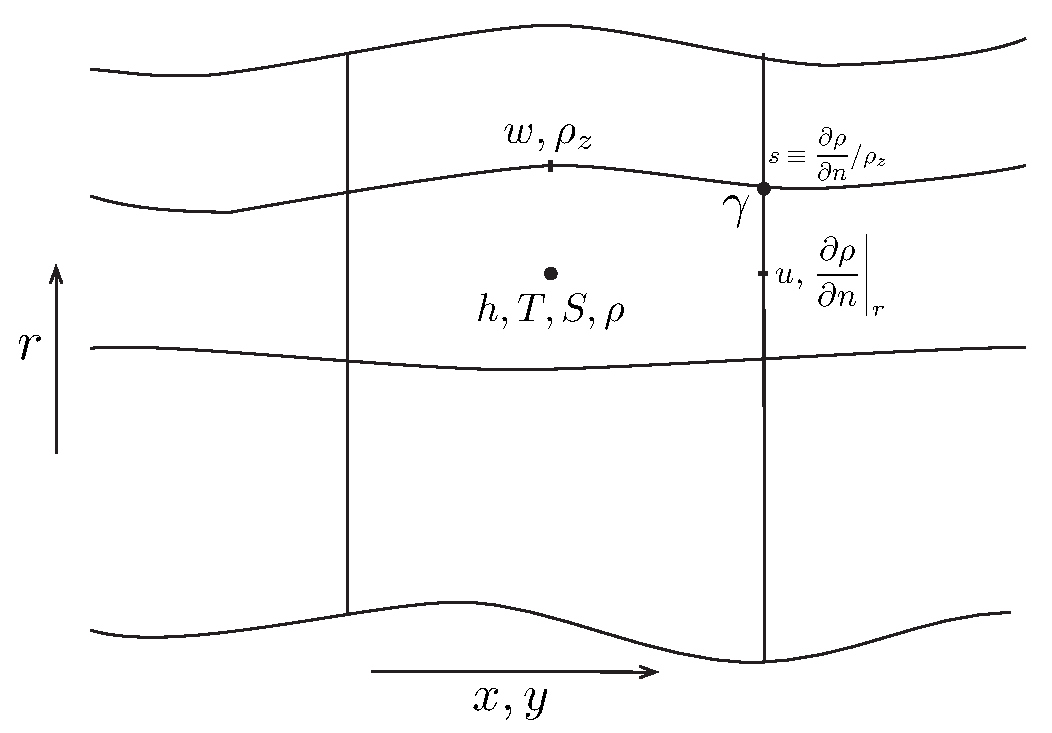
\includegraphics{variable-placement.pdf}}
  \caption{The placement of the discrete variables}
  \label{fig:1}
\end{figure}
We assume that a general vertical coordinate $r$ is in use. In the 3D
MPAS-O model, the scalar variables $h,\, T,\, S,\, \rho$ etc.~are
defined at the cell centers and in the middle of the layers. The
horizontal normal velocity component $u$ is defined at the cell edges
and in the middle of the layers. The vertical transport velocity $w$
is defined at the cell centers and at the layer interfaces. The normal
derivative of the density field is then most conveniently calculated
on the cell edges and in the middle of the layers. The vertical
derivative $\rho_z$ is most conveniently calculated at the cell
centers and at the layer interfaces. The calculations of the normal
component of the slope $\bs{s}$ of the constant density surfaces or
the calculations of the normal component of the vector $\bs{\gamma}$
involve both $\rho_z$ and $\p\rho/\p\mathrm{n}$, which suggests that
$s$ and/or $\gamma$ should be specified on the cell edges and at the
layer interfaces. 

 \section{Computation steps in the GM module}
\label{sec:sequence-actions-gm}
\begin{itemize}
\item  Step 1. Compute $\frac{\p\rho}{\p n}|_r$ at cell edge and layer center.
\item Step 2. Compute $\frac{\p\rho}{\p z}$ at cell center and layer
  interface.
\item Step 3. Compute $(\p z/\p n)|_r$ at cell edge and layer center.
\item Step 4. Interpolate $\frac{\p\rho}{\p z}$ to cell edge and layer
  interface.
\item Step 5. Interpolate $\frac{\p\rho}{\p z}$ to cell center and
  middle of layers.
\item Step 6. Interpolate $\frac{\p\rho}{\p n}|_r$ to cell edge and
  layer interface.
\item Step 7. Interpolate $(\p z/\p n)|_r$ to cell edge and layer
  interface.
\item Step 8a. Compute the slope $S$ according to \eqref{eq:9} and then the uBolusGM according to
  \eqref{eq:12}. Or
\item Step 8b. Compute the stream function $\gamma$ according to
  \eqref{eq:19}--~\eqref{eq:20}, and uBolusGM according to
  \eqref{eq:13}.
\item Step 9. Compte $\tilde S$ (i.e.~{\tt slope}) at cell edge and layer interface
  according to \eqref{eq:56}.
\item 10. Compute $K_{33}$ according \eqref{eq:57}.
\item 11. Pass out uBolusGM, $\tilde S$ and $K_{33}$.
\end{itemize}

\subsection{Additional computation steps in {\tt 
    ocn\_tracer\_hmix\_tend}}
\label{sec:addit-comp-steps}
\begin{itemize}
\item Interpolate {\tt slope} to cell edge and middle of layers.
\item Interpolate $(\p\varphi/\p n)|_r$ to cell edge and layer interface.
\item Comute  $\nabla_r\cdot\left(\tilde{\mathbf{S}}\frac{\p\varphi}{\p
      z}\right)$ according to \eqref{eq:58}.
\item Compute $\tilde{\mathbf{S}}\cdot\nabla_r\varphi$ according to \eqref{eq:59}.
\end{itemize}

%-----------------------------------------------------------------------

\chapter{Testing}\label{cha:testing}
The goal of the testing process is to ensure that the implementation
is working as it is intended by the design laid out in previous
sections. We particularly point out that the testing is not about
whether GM is a good mesoscale eddy parametrization.

\section{Testing and Validation: the vertical boundary value problem}
Date last modified: 2012/09/20 \\
Contributors: Qingshan Chen and Todd Ringler\\

The boundary value problem \eqref{eq:19}-~\eqref{eq:20} will also be
implemented in Matlab. The Matlab will be evaluated based on exact solutions. The solver will then be implemented into MPAS, but run in diagnostic mode only. We will configure an ocean basin such that every column matches the Matlab testing condition and insure that we obtain the same results as the Matlab code.

\section{Testing and Validation: diagnostic isopycnal setting}
Date last modified: 2012/09/20 \\
Contributors: Qingshan Chen and Todd Ringler\\

A three-layer isopycnal model should be configured and run, with GM
being implemented based on the layer thickness and on the isopycnal
slopes. These two different implementations should produce close
results in terms of the output of the bolus velocities and the
overall model outputs. In these two cases, the bolus velocities will be diagnostics only (i.e. will not feedback into the model solution).

\section{Testing and Validation: isopycnal setting}
Date last modified: 2012/09/20 \\
Contributors: Qingshan Chen and Todd Ringler\\

A three-layer isopycnal model should be configured and run, with GM
being implemented based on the layer thickness and on the isopycnal
slopes. These two different implementations should produce close
results in terms of the output of the bolus velocities and the
overall model outputs. In these two cases, the bolus velocities will be included into the model transport velocity. This will test the stability of the new bolus velocity computation.

\section{Testing and Validation: the low-res $z$-level or $z^\ast$ settings}
Date last modified: 2012/09/20 \\
Contributors: Qingshan Chen and Todd Ringler\\

A 125km $z$-level model of the ACC and a 125km $z^\ast$ of the same
model should be run with and without the GM turned on. The GM closure
is expected to lead to flatter isopycnal slopes and slower jets.


\section{Testing and Validation: Redi isopycnal diffusion}
Date last modified: 2012/09/20 \\
Contributors: Qingshan Chen and Todd Ringler\\

????



%-----------------------------------------------------------------------
\bibliographystyle{plain}
\bibliography{gm-references}


\end{document}
